%
%===============>>  Порядин Модуль 8 <<=============
%=
\setmodule{8}

%BEGIN_FOLD % ====>>_____ Занятие 1 _____<<====
\begin{class}[number=1]
	\begin{listofex}
		\item Решите уравнения: 
			\begin{tasks}(2)
			\task \( x^3=6x^2+7x \)
			\task \( x^3=x^2-7+7 \)
			\task! \( (x-2)(x-3)(x-4)=(x-3)(x-4)(x-5) \)
			\task \( x(x^{2}+4x+4)=3(x+2) \)
			\task \( (x+5)^{3}=25(x+5)\)
		\end{tasks} 
		\item Решите неравенства:
		\begin{tasks}(2)
			\task \( \dfrac{(x-3)(x-4)}{x-5}\ge0 \)
			\task \( \dfrac{(x+1)(x-1)}{x-3}<0 \)
			\task \( \dfrac{(x-0)(x-3)}{x+4}>0 \)
			\task \( \dfrac{x}{(x+1)(x-8)}\le0 \)
		\end{tasks}
		\item Постройте график функции \( y=5-\dfrac{x^4-x^3}{x^2-x} \) и определите, при каких значениях \( m \) прямая \( y=m \) имеет с графиком ровно две общие точки.
	\end{listofex}
\end{class}
%END_FOLD

%BEGIN_FOLD % ====>>_____ Занятие 2 _____<<====
\begin{class}[number=2]
	\begin{listofex}
		\item .
	\end{listofex}
\end{class}
%END_FOLD

%BEGIN_FOLD % ====>>_ Домашняя работа 1 _<<====
\begin{homework}[number=1]
	\begin{listofex}
		\item Решите неравенства:
		\begin{tasks}(2)
			\task \( \dfrac{(x+3)(x+4)}{x+5}\le0 \)
			\task \( \dfrac{x}{(x-3)(x+4)}>0 \)
			\end{tasks}
		\item Постройте график функции \( y=\dfrac{(x^2-4)(x^2-4x+3)}{x^2-3x+2} \) и определите, при каких значениях \( m \) прямая \( y=m \) имеет с графиком ровно одну общую точку.
	\end{listofex}
\end{homework}
%END_FOLD

%BEGIN_FOLD % ====>>_____ Занятие 3 _____<<====
\begin{class}[number=3]
	\begin{listofex}
		\item На экзамене \( 25 \) билетов, Сергей не выучил \( 3 \) из них. Найдите вероятность того, что ему попадётся выученный билет.
		\item Телевизор у Саши сломался и показывает только один случайный канал. Саша включает телевизор. В это время по пятнадцати каналам из пятидесяти показывают кинокомедии. Найдите вероятность того, что Саша попадет на канал, где комедия не идет.
		\item В фирме такси в данный момент свободно \( 15 \) машин: \( 3 \) чёрных, \( 6 \) жёлтых и \( 6 \) зелёных. По вызову выехала одна из машин, случайно оказавшаяся ближе всего к заказчику. Найдите вероятность того, что к нему приедет жёлтое такси.
		\item В каждой пятой банке кофе согласно условиям акции есть приз. Призы распределены по банкам случайно. Галя покупает банку кофе в надежде выиграть приз. Найдите вероятность того, что Галя не найдёт приз в своей банке.
		\item В среднем из каждых \( 80 \) поступивших в продажу аккумуляторов \( 76 \) аккумуляторов заряжены. Найдите вероятность того, что купленный аккумулятор не заряжен.
		\item Для экзамена подготовили билеты с номерами от \( 1 \) до \( 25 \). Какова вероятность того, что наугад взятый учеником билет имеет номер, являющийся двузначным числом?
		\item В мешке содержатся жетоны с номерами от \( 2 \) до \( 51 \) включительно. Какова вероятность, того, что номер извлеченного наугад из мешка жетона является однозначным числом?
		\item В денежно-вещевой лотерее на \( 100000 \) билетов разыгрывается \( 1300 \) вещевых и \( 850 \) денежных выигрышей. Какова вероятность получить вещевой выигрыш?
		\item В чемпионате по футболу участвуют \( 16 \) команд, которые жеребьевкой распределяются на \( 4 \) группы: \( A \), \( B \), \( C \) и \( D \). Какова вероятность того, что команда России не попадает в группу \( A \)?
		\item В группе из \( 20 \) российских туристов несколько человек владеют иностранными языками. Из них пятеро говорят только по-английски, трое только по-французски, двое по-французски и по-английски. Какова вероятность того, что случайно выбранный турист говорит по-французски?
		\item Стас, Денис, Костя, Маша, Дима бросили жребий --- кому начинать игру. Найдите вероятность того, что начинать игру должна будет девочка.
		\item В лыжных гонках участвуют \( 11 \) спортсменов из России, \( 6 \) спортсменов из Норвегии и \( 3 \) спортсмена из Швеции. Порядок, в котором спортсмены стартуют, определяется жребием. Найдите вероятность того, что первым будет стартовать спортсмен из России.
		\item Из каждых \( 1000 \) электрических лампочек \( 5 \) бракованных. Какова вероятность купить исправную лампочку?
		\item Определите вероятность того, что при бросании кубика выпало число очков, не большее \( 3 \).
		\item Игральную кость бросают дважды. Найдите вероятность того, что оба раза выпало число, большее \( 3 \).
		\item Игральную кость бросают дважды. Найдите вероятность того, что сумма двух выпавших чисел равна \( 4 \) или \( 7 \).
	\end{listofex}
\end{class}
%END_FOLD

%BEGIN_FOLD % ====>>_____ Занятие 4 _____<<====
\begin{class}[number=4]
	\begin{listofex}
		\item Биссектрисы углов \( N \) и \( M \) треугольника \( MNP \) пересекаются в точке \( A \). Найдите \( \angle NAM \), если \( \angle N=84\degree \), а \( \angle M=42\degree \).
		\item Диагональ прямоугольника образует угол \( 51\degree \) с одной из его сторон. Найдите острый угол между диагоналями этого прямоугольника. Ответ дайте в градусах.
		\item
		\begin{minipage}[t]{\bodywidth}
			Углы, отмеченные на рисунке одной дугой, равны. Найдите угол \( \alpha \). Ответ дайте в градусах.
		\end{minipage}
		\hspace{0.02\linewidth}
		\begin{minipage}[t]{\picwidth}
			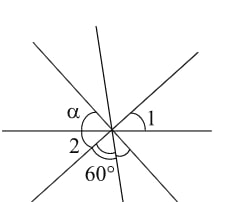
\includegraphics[align=t, width=0.8\linewidth]{../../../../../exercises/lists/pics/leontevaM7H2-1}
		\end{minipage}
		\item
		\begin{minipage}[t]{\bodywidth}
			Углы, отмеченные на рисунке одной дугой, равны. Найдите угол \( \alpha \). Ответ дайте в градусах.
		\end{minipage}
		\hspace{0.02\linewidth}
		\begin{minipage}[t]{\picwidth}
			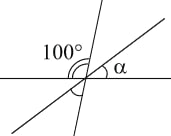
\includegraphics[align=t, width=0.8\linewidth]{../../../../../exercises/lists/pics/leontevaM7H2-2}
		\end{minipage}
		\item 
		\begin{minipage}[t]{\bodywidth}
			На плоскости даны четыре прямые. Известно, что \( \angle 1 = 120^{\circ} \), \( \angle 2 = 60^{\circ} \), \( \angle 3 = 55^{\circ} \). Найдите \( \angle 4 \). Ответ дайте в градусах.
		\end{minipage}
		\hspace{0.02\linewidth}
		\begin{minipage}[t]{\picwidth}
			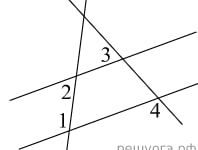
\includegraphics[align=t, width=0.8\linewidth]{../../../../../exercises/lists/pics/leontevaM7H2-3}
		\end{minipage}		
		\item На сторонах угла \( BAC \) и на его биссектрисе отложены равные отрезки \( AB \), \( AC \) и \( AD \). Величина угла \( BDC \) равна \( 160\degree \). Определите величину угла \( BAC \).
		\item В треугольнике \( ABC \) углы \( A \) и \( C \) равны \( 40\degree \) и \( 60\degree \) соответственно. Найдите угол между высотой \( BH \) и биссектрисой \( BD \).
		\item Центральный угол \( AOB \) опирается на хорду \( AB \) длиной \( 6 \). При этом угол \( OAB \) равен \( 60\degree \). Найдите радиус окружности.
		\item В окружности с центром в точке \( O \) проведены диаметры \( AD \) и \( BC \), угол \( OCD \) равен \( 30\degree \). Найдите величину угла \( OAB \).
		\item Найдите градусную меру тупого центрального угла \( MON \), если известно, \( NP \) --- диаметр, а градусная мера угла \( MNP \) равна \( 18\degree \).
		\item Найдите вписанный угол \( DEF \), если градусные меры дуг \( DE \) и \( EF \) равны \( 150\degree \) и \( 68\degree \) соответственно.
		\item Найдите градусную меру угла \( ACB \), если известно, что \( BC \) является диаметром окружности, а градусная мера центрального угла \( AOC \) равна \( 96\degree \).
		\item В окружности с центром \( O \) \( AC \) и \( BD \) --- диаметры. Угол \( ACB \) равен \( 26\degree \). Найдите угол \( AOD \). Ответ дайте в градусах.
		\item Прямоугольный треугольник с катетами \( 5 \) см и \( 12 \) см вписан в окружность. Чему равен радиус этой окружности?
		\item Точки \( A \) и \( B \) делят окружность на две дуги, длины которых относятся как \( 9:11 \). Найдите величину центрального угла, опирающегося на меньшую из дуг. Ответ дайте в градусах.
		\item Величина центрального угла \( AOD \) равна \( 110\degree \). Найдите величину вписанного угла \( ACB \). Ответ дайте в градусах.
		\item Точки \( A \), \( B \), \( C \) и \( D \) лежат на одной окружности так, что хорды \( AB \) и \( CD \) взаимно перпендикулярны, а угол \( BDC=25\degree \) . Найдите величину угла \( ACD \).
	\end{listofex}
\end{class}
%END_FOLD

%BEGIN_FOLD % ====>>_ Домашняя работа 2 _<<====
\begin{homework}[number=2]
	\begin{listofex}
		\item Телевизор у Любы сломался и показывает только один случайный канал. Люба включает телевизор. В это время по двадцати пяти каналам из пятидесяти показывают кинокомедии. Найдите вероятность того, что Люба попадет на канал, где комедия не идет.
		\item В среднем из каждых \( 60 \) поступивших в продажу аккумуляторов \( 58 \) аккумуляторов заряжены. Найдите вероятность того, что купленный аккумулятор не заряжен.
		\item Для экзамена подготовили билеты с номерами от \( 1 \) до \( 25 \). Какова вероятность того, что наугад взятый учеником билет имеет номер, являющийся двузначным числом?
		\item 
		\begin{minipage}[t]{\bodywidth}
		 Найдите величину угла \( AOE \), если \( OE \) --- биссектриса угла \( AOC \), \( OD \) --- биссектриса угла \( COB \).
		\end{minipage}
		\hspace{0.02\linewidth}
		\begin{minipage}[t]{\picwidth}
			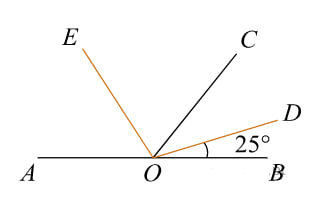
\includegraphics[align=t, width=0.8\linewidth]{../../../../../exercises/lists/pics/poryadinM8H2}
		\end{minipage}	
		\item В окружности с центром в точке \( O \) проведены диаметры \( AD \) и \( BC \), угол \( OAB \) равен \( 25\degree \). Найдите величину угла \( OCD \).
		\item Отрезки \( AC \) и \( BD \) --- диаметры окружности с центром \( O \). Угол \( ACB \) равен \( 23\degree \). Найдите угол \( AOD \). Ответ дайте в градусах.
		\item На окружности с центром \( O \) отмечены точки \( A \) и \( B \) так, что \( \angle AOB=39\degree \). Длина меньшей дуги \( AB \) равна \( 65 \). Найдите длину большей дуги.
		\item Центр окружности, описанной около треугольника \( ABC \), лежит на стороне \( AB \). Найдите угол \( ABC \), если угол \( BAC \) равен \( 9\degree \). Ответ дайте в градусах.
	\end{listofex}
\end{homework}
%END_FOLD

%BEGIN_FOLD % ====>>_____ Занятие 5 _____<<====
\begin{class}[number=5]
	\begin{listofex}
		\item Занятие 5
	\end{listofex}
\end{class}
%END_FOLD

%BEGIN_FOLD % ====>>_____ Занятие 6 _____<<====
\begin{class}[number=6]
	\begin{listofex}
		\item Занятие 6
	\end{listofex}
\end{class}
%END_FOLD

%BEGIN_FOLD % ====>>_ Домашняя работа 3 _<<====
\begin{homework}[number=3]
	\begin{listofex}
		\item .
	\end{listofex}
\end{homework}
%END_FOLD

%BEGIN_FOLD % ====>>_____ Занятие 7 _____<<====
\begin{class}[number=7]
	\title{Подготовка к проверочной}
	\begin{listofex}
		\item Занятие 7
	\end{listofex}
\end{class}
%END_FOLD

%BEGIN_FOLD % ====>>_ Проверочная работа _<<====
\begin{exam}
	\begin{listofex}
		\item Проверочная
	\end{listofex}
\end{exam}
%END_FOLD